\pagebreak
\section{Serveur}
\label{chapter:api}

Cette section est entièrement dédiée à la conception du \gls{backend} de \texttt{SourceCode}.
Puisque cette partie est l'extrême opposé de la précédente (cf. section \ref{chapter:client}), nous l'aborderons par sa réalisation technique, en nous concentrant sur l'essentiel.

\subsection{Structure du projet}

Pour répondre aux besoins exprimés en chapitre \ref{chapter:analyseDesBesoins} et sur base de nos choix (cf. section \ref{section:choixTechnologiques}), nous avons élaboré la présente structure :

% Généré avec tree sur Windows et https://carbon.now.sh/
\begin{figure}[H]
    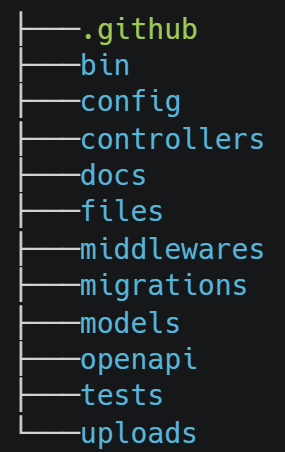
\includegraphics[width=\textwidth,height=0.25\textheight,keepaspectratio]{images/serveur/tree_folders.png}
    \centering
    \caption[SourceCode : Arborescence de l'API]{Arborescence de l'\Gls{api}}
    \label{fig:arborenceAPI}
\end{figure}

Cette structure ne vous est peut-être pas inconnue, car il s'agit de la structure officielle de Sequelize\footnote{
    \url{https://github.com/sequelize/cli} - command "sequelize init"
}, sur laquelle nous avons ajouté quelques dossiers :

% A voir s'il faut minimiser l'itemize
% nosep,noitemsep,topsep=0pt,partopsep=0pt,after=\vspace*{2pt}
\begin{itemize}
    \item openapi : nos fichiers \Gls{oas}, utilisés par openapi-enforcer (cf. figure \ref{fig:OASEnforcer})
    \item controllers : nos fichiers chargés de répondre aux requêtes \textbf{HTTP}, utilisés par openapi-enforcer (cf. figure \ref{fig:OASEnforcer})
    \item tests : nos tests pour valider l'implémentation (cf. chap TODO)
    \item docs : la documentation de l'\Gls{api} en \textbf{HTML}\footnote{
        Celle-ci est automatiquement publiée sur 
        \href{https://sourcecodeoer.github.io/sourcecode\_api/}{https://sourcecodeoer.github.io/sourcecode\_api/}.
        Pour la générer en local, cela se fait via la commande : 
        npx redoc-cli bundle api.yml -o docs/index.html 
    } (cf. figure \ref{fig:exampleDoc} pour un exemple)
    \item upload / files : resp. lieu de stockage des fichiers importés / stockés 
    \item .github : nos scripts d'automatisation (cf. section TODO) 
    \item bin : du code n'entrant dans aucun autre dossier
\end{itemize}

\pagebreak
\subsection{Points clés de l'implémention}

\subsubsection{Paramétrisation de l'\Gls{api}}

Comme révélé en section \ref{section:AnalyseNonFonctionnelle}, il convient d'accorder un certain contrôle aux utilisateurs finaux.
Une manière de configurer une telle application est d'utiliser des \glspl{envvar}, 
qui permettent, contrairement à d'autres approches (comme les fichiers de configuration \textbf{JSON}, \textbf{YAML}, ...), 
de changer de valeur directement, sans éteindre/rédémarrer l'application par exemple. \\

Nous avons accordé les possibilités suivantes (la liste détaillée des \glspl{envvar} est disponible dans le fichier README.MD) :

\begin{itemize}
    \item Changer le port utilisé par l'\Gls{api}
    \item Changer l'URI pour se connecter à la base de données
    \item Changer la politique de traçabilité (cf. section 4.2 - partie "Sécurité")
    \item Changer la durée de validité du token \textbf{JWT} (cf. section \ref{section:choixTechnologiques})
\end{itemize}

\subsubsection{Documentation de l'\Gls{api}}

De manière synthétique, \Gls{oas}\footnote{
    Pour des exemples concrets, veuillez vous référer au fichier api.yml et le dossier openapi
} a été plébiscité pour les raisons suivantes :

\begin{itemize}
    \item Peut être utilisé par des outils divers pour de multiples finalités :
    \begin{itemize}[nosep,noitemsep,topsep=0pt,partopsep=0pt,after=\vspace*{2pt}]
        \item apporter des fonctionnalités supplémentaires / construire un projet plus rapidement, comme OpenAPI-enforcer (cf. figure \ref{fig:OASEnforcer})
        \item pour générer de la documentation (cf. figure \ref{fig:exampleDoc}), comme Redoc\footnote{
            \url{https://github.com/Redocly/redoc}
        }
    \end{itemize}
    \item Non dépendant du code : de ce fait, plus facile à maintenir et à faire évoluer
\end{itemize}

\begin{figure}[H]
    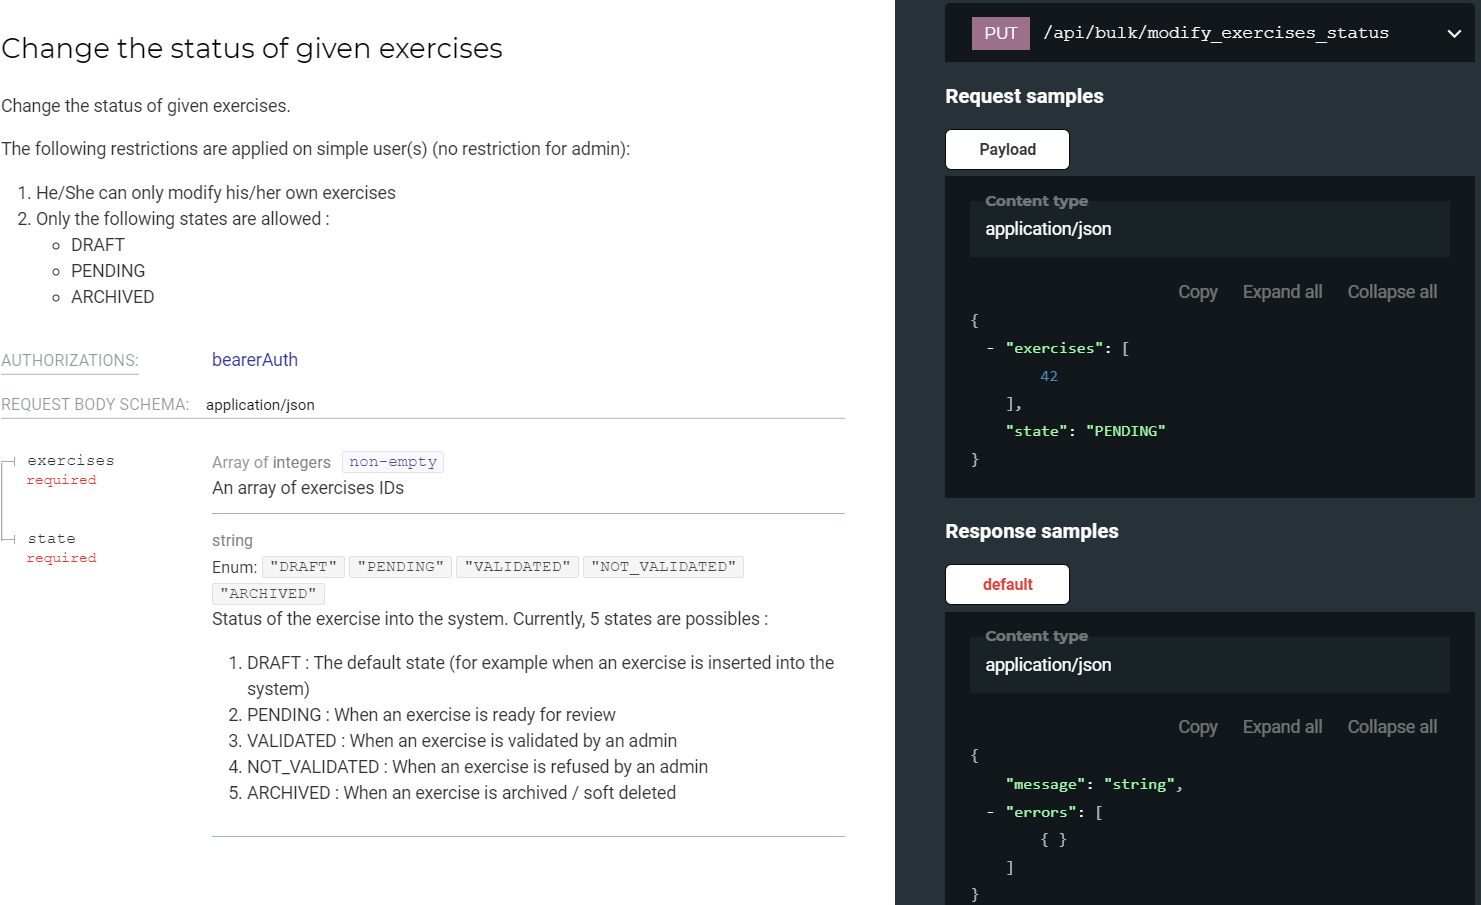
\includegraphics[width=\textwidth,height=0.44\textheight,keepaspectratio]{images/serveur/doc_example.png}
    \centering
    \caption{Exemple de documentation \textbf{HTML} générée sur base de fichiers \Gls{oas}}
    \label{fig:exampleDoc}
\end{figure}

\pagebreak
\subsubsection{\Glspl{middleware}}

Pour rappel (cf section \ref{section:choixTechnologiques}), Express a été le "squelette" sur lequel nous avons construit notre application.
Une de ses particularités est l'usage de \glspl{middleware}\footnote{
    Par exemple, ceux en section \ref{section:choixTechnologiques} : Passport.js et OpenAPI-enforcer
} dont nous pouvons expliquer le fonctionnement général par le biais de cette illustration :

\begin{figure}[H]
    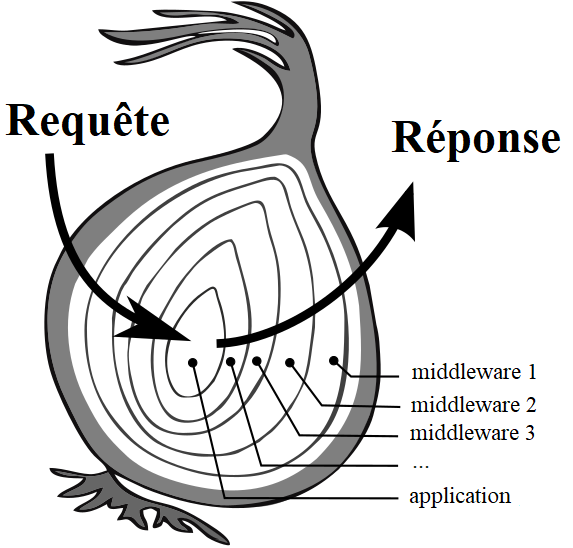
\includegraphics[width=\textwidth,height=0.25\textheight,keepaspectratio]{images/serveur/middleware_onion.png}
    \centering
    \caption{\Glspl{middleware} : modèle de l'oignon}
    \label{fig:middlewareOnion}
\end{figure}

\begin{itemize}[nosep,noitemsep,topsep=0pt,partopsep=0pt,after=\vspace*{2pt}]
    \item La requête est interceptée par le serveur.
    \item La requête traverse successivement chaque "couche" (\gls{middleware} 1, 2, ...) jusqu'à atteindre le cœur de l'application, 
    à condition qu'il n'y ait pas eu d'erreurs lors du parcours.
    \item Quelque soit la situation, une réponse est toujours envoyée au client de la requête.
\end{itemize}

La grande force de cette approche est qu'elle permet de déléguer\footnote{
    Par exemple, l'authentification (cf. section \ref{section:AnalyseNonFonctionnelle}), la validation des requêtes (cf. figure \ref{fig:OASEnforcer}) ...
} et se concentrer ainsi sur l'essentiel. Il est également possible de combiner plusieurs \glspl{middleware} en un seul dans une même "couche", par des \glspl{library} comme connect-chain-if
\footnote{
    \url{https://www.npmjs.com/package/connect-chain-if}
}.

\subsubsection{Recherche par \glspl{tag}}
\label{section:SearchTagImpl}

Pour rappel, nous avions abordé au chapitre \ref{chapter:analyseDesBesoins} (cf. table \ref{tab:fichesWithTagExample}) la problématique de la recherche et de la solution théorique que nous envisagions.
Notre implémentation repose sur un champ précalculé\footnote{
    Par souci de performances, il est préférable d'avoir cette information directement, plutôt que la calculer sur la table intermédiaire entre les \glspl{fiche} et les \glspl{tag} à chaque fois.
}, de type tableau d'entiers (ex: [1,2,3] signifie que la \gls{fiche} dispose des \glspl{tag} avec les identifiants 1, 2 et 3).
Avec notre implémentation (cf. code \ref{code:searchTags}), notre format de requête
\footnote{
   Les crochets ayant la même signification que les parenthèses de la \textbf{FNC} ; 
   le $\lnot$ d'un entier s'encode avec le même entier, mais avec un symbole négatif ; 
   le $\land$ s'effectue sur les éléments du premier niveau tandis que le $\lor$ s'effectue lui sur le 2e niveau
} et les "scopes" en Sequelize (cf. section \ref{section:choixTechnologiques}), 
il est possible de l'appliquer à l'exemple en table \ref{tab:fichesWithTagExample}, avec les 3 mêmes requêtes que nous avions utilisées :

\begin{table}[H]
    \centering
    \begin{tabular}{|c|c|c|c|}
        \hline
            recherche / \gls{fiche} & F1 & F2 & F3 \\ \hline
            [ [1, 2] ] & \checkmark  & \checkmark  &    \\ \hline
            [2, [-1, -2] ] &    & \checkmark  &   \\ \hline
            [-3] & \checkmark &    & \checkmark   \\ \hline
    \end{tabular}
    \caption{Solution technique de la recherche par \glspl{tag}}
    \label{tab:fichesWithTagImpl}
\end{table}

% DIVERS
% - Docker (en annexe, les deux docker-compose)
% - CLI : max une page ou deux (expliquer ce qu'il y a dedans, en ref l'annexe A)
\pagebreak
\section{Divers}
\label{chapter:solutionDivers}

Dans cette section, nous aborderons quelques éléments secondaires de \texttt{SourceCode}.
En effet, en dehors du développement, il existe bien d'autres facettes importantes du cycle de vie\footnote{
    En anglais, ce terme est connu sous le nom de "software lifecycle". (\url{https://web.maths.unsw.edu.au/~lafaye/CCM/genie-logiciel/cycle-de-vie.htm})
} d'un logiciel : le \gls{deploiement} / la \gls{maintenance}  ...

\subsection{\texorpdfstring{\Gls{cli}}{CLI}}

Comme nous l'évoquions précédemment (cf. annexe \ref{annexe:AnalyseBiblio}), il convient de disposer d'outils pour indexer / mettre en ligne un nombre conséquent de 
\glspl{resinfo}, provenant de diverses sources, en un minimum de temps. C'est pour répondre à ce besoin que nous avons développé un \Gls{cli}, sur base du framework Yargs
(cf. section \ref{section:choixTechnologiques})\footnote{
    % TODO Code B1
    Comme le montre le point d'entrée du \Gls{cli}, à savoir "index.js" (que nous avons inclus dans l'annexe ???), il sera aisé d'ajouter de nouvelles commandes à l'avenir.
}.

% TODO illustration by Alexandre
% TODO texte pour introduire figure d'Alexandre

% TODO code B2

Chaque commande disposant 
\begin{itemize}
    \item La possibilité d'utiliser 
\end{itemize}

Par respect de la norme que nous avons crée (cf. annexe \ref{annexe:AnalyseBiblio}), nous avons également adopté le \textbf{JSON} et les mêmes conventions d'écriture 
pour les fichiers d'entrée / de sortie des différentes commandes, à quelques exceptions près que nous avons détaillé dans le fichier README.MD. 

\pagebreak
\subsection{Docker}
\subsection{Github Actions}

permettant de réaliser en outre du \gls{ci_cd}

